\documentclass[main.tex]{subfiles}

\begin{document}

\begin{q}{1}
Consider the planet Mars. Calculate its relative distance by using the following
observational data. Do not use Kepler's laws of planetary motion and Newton's
law of universal gravitation (assume that they have yet to be discovered).

\noindent\textit{Hint: Consider the reference frame in which the Sun and Earth
are not moving. Find the angle subtended at the Sun by two of the phenomena. Use
trigonometry to calculate Mars' relative distance.}

\begin{table}[h!]
    \centering
    \begin{tabular}{|c|c|}
    \hline
    \textbf{Date} & \textbf{Phenomenon} \\
    \hline
    2023-11-18 & Conjunction \\
    2024-10-14 & Western quadrature \\
    2025-01-16 & Opposition \\
    2025-04-21 & Eastern quadrature \\
    \hline
    \end{tabular}
    \caption*{Reference:
    \href{https://eco.mtk.nao.ac.jp/cgi-bin/koyomi/cande/phenomena_en.cgi}{https://eco.mtk.nao.ac.jp/cgi-bin/koyomi/cande/phenomena\_en.cgi}}
    \end{table}
\end{q}

\begin{sol}
First, we define the average distance the Earth and Mars are from the Sun as $1$
and $x$ astronomical unit(s) respectively where $x > 1$. Assuming that the
orbits of Earth and Mars around the Sun is perfectly circular, we obtain the
following geometric construction.
\begin{figure}[h!]
    \centering
    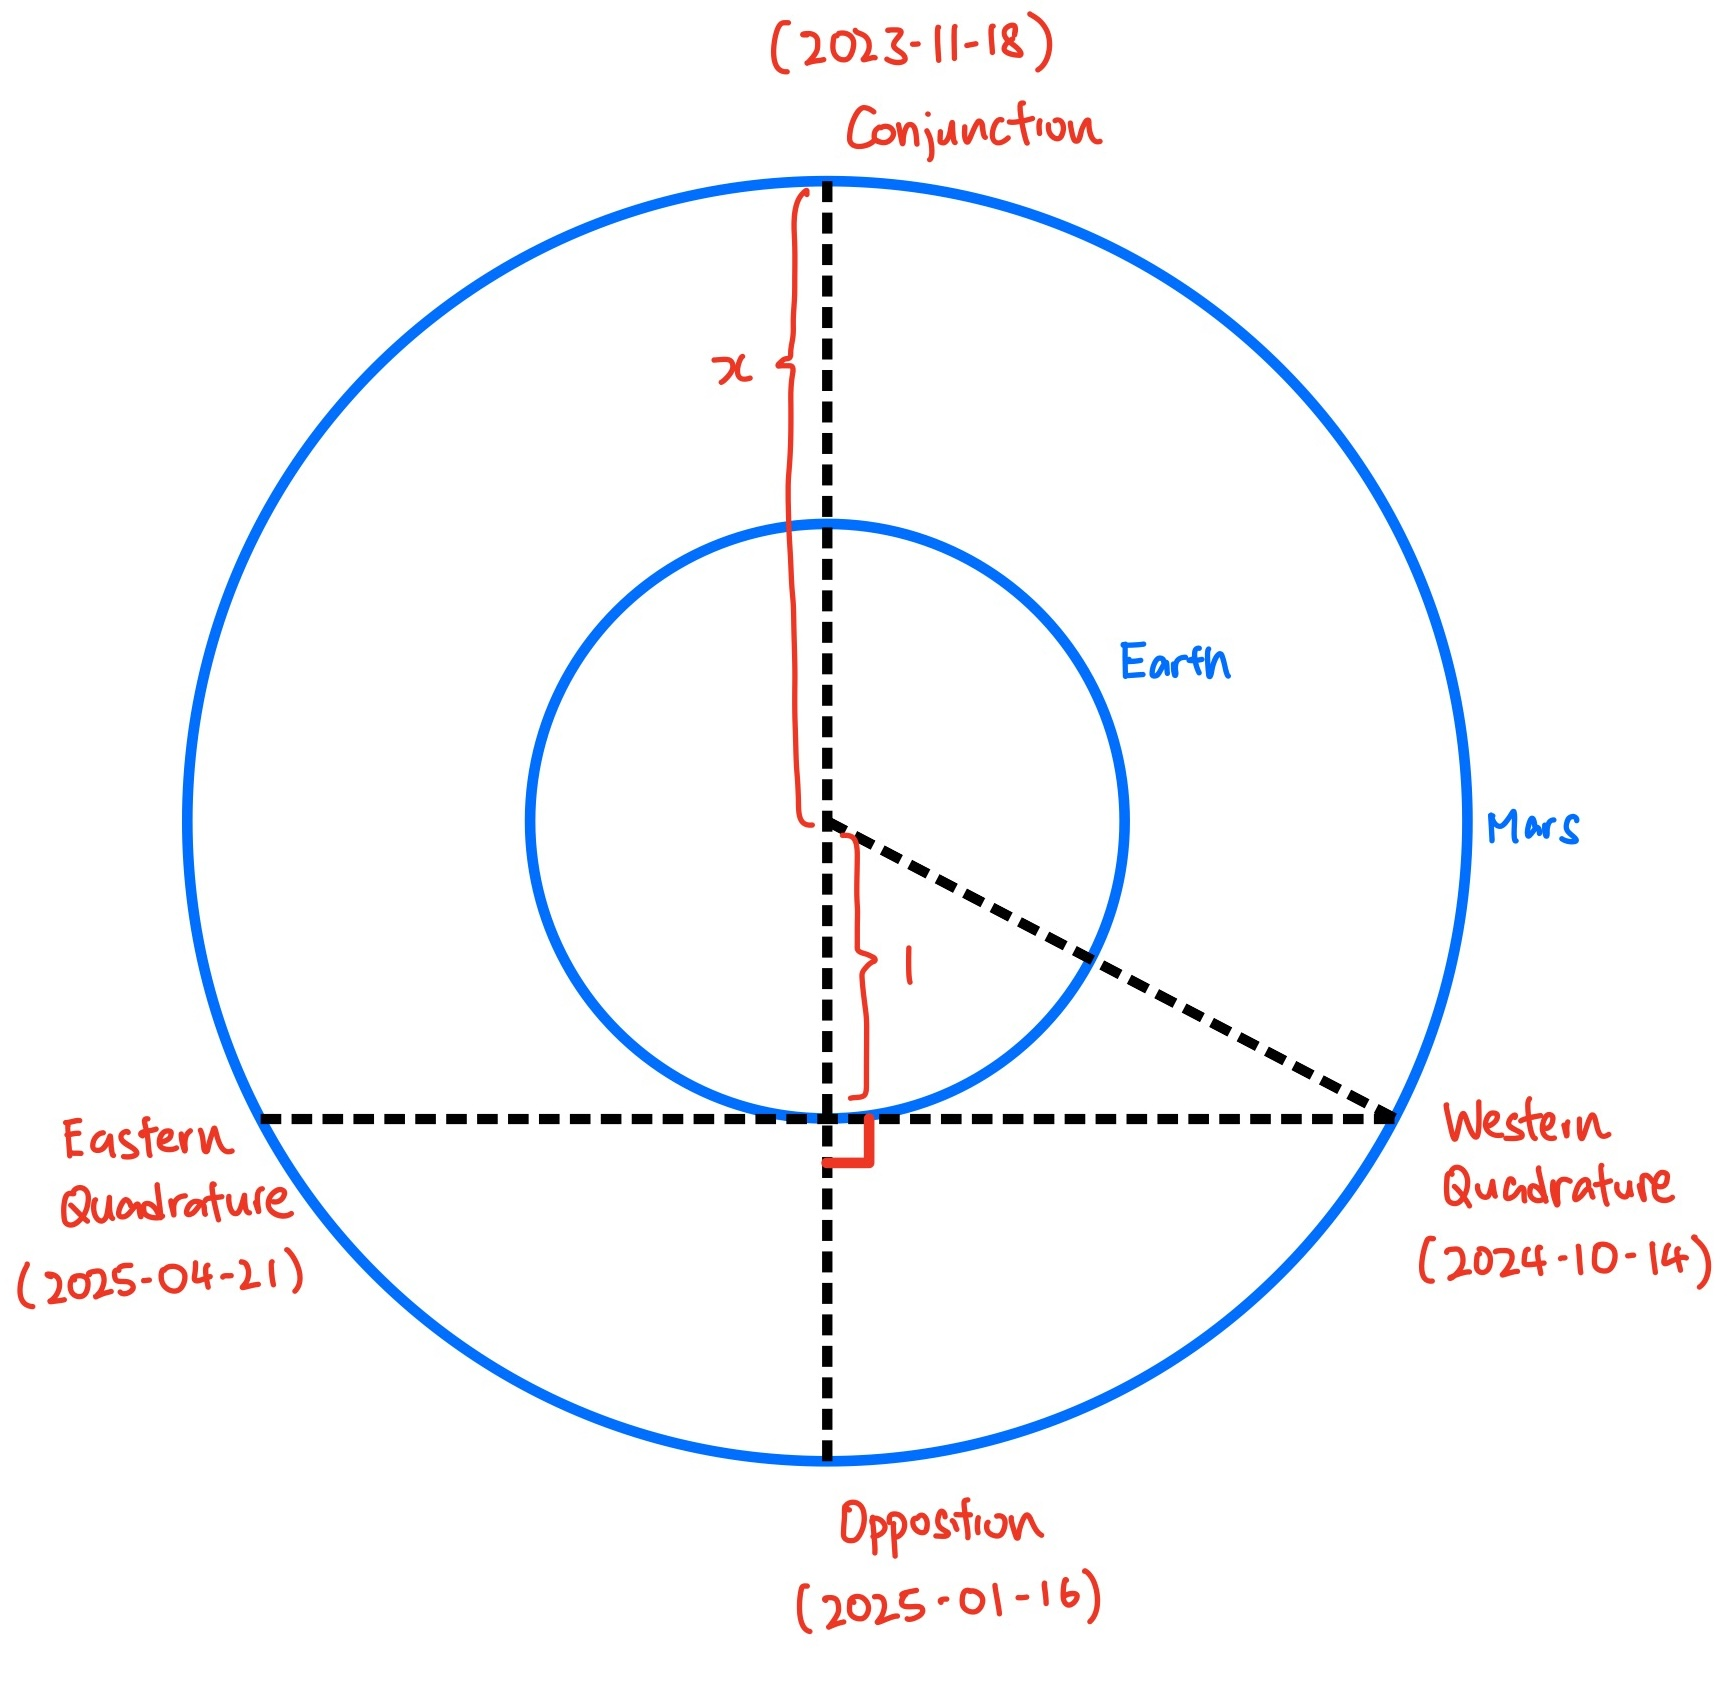
\includegraphics[width=0.5\textwidth]{figure1}
\end{figure}

\newpage\noindent Consider Mars' motion around the Sun in the fixed Sun-Earth
stationary frame, Mars should have a constant angular velocity. Hence,
\begin{equation}
    \omega = \frac{2\pi}{t_{\text{synodic}}} = \frac{\Delta\theta}{\Delta t}\qquad \implies \qquad\Delta \theta \propto \Delta t.
\end{equation}
As such,
\begin{equation}
    \Delta \theta = \omega \Delta t = \frac{2\pi}{t_{\text{synodic}}} \Delta t = \frac{2\pi}{t_{\text{synodic}}} \paren{t_{\text{eastern quadrature}} - t_{\text{western quadrature}}},
\end{equation}
where if we consider the Sun-Earth-Mars (western quadrature) right triangle such
that the angle subtended between the Sun-Mars line and the Sun-Earth line is
$\varphi$, we have
\begin{equation}
    \varphi = \frac{\Delta\theta}{2} = \frac{\pi}{t_{\text{synodic}}} \paren{t_{\text{eastern quadrature}} - t_{\text{western quadrature}}}\qquad \text{and} \qquad\cos\varphi = \frac{1}{x}.
\end{equation}
Given the date where Mars is in conjunction and in opposition with respect to
Earth,
\begin{equation}
    t_{\text{synodic}} = 2\paren{t_{\text{opposition}} - t_{\text{conjunction}}}.
\end{equation}
we thus have
\begin{equation}
    \begin{split}
        x &= \frac{1}{\cos\sparen{\frac{\pi}{2\paren{t_{\text{opposition}} - t_{\text{conjunction}}}}\paren{t_{\text{eastern quadrature}} - t_{\text{western quadrature}}}}}\\
        &= \frac{1}{\cos\sparen{\frac{\pi}{2\paren{\SI{425}{\day}}}\paren{\SI{189}{\day}}}} \approx \SI{1.3059}{\au}\\
        &\approx \SI{1.31}{\au}\quad\paren{\text{3 s.f.}}
    \end{split}
\end{equation}
Alternatively, if we choose $t_{\text{synodic}} = \SI{780}{\day}$, we have,
\begin{equation}
    \begin{split}
        x &= \frac{1}{\cos\sparen{\frac{\pi}{t_{\text{synodic}}}\paren{t_{\text{eastern quadrature}} - t_{\text{western quadrature}}}}} = \frac{1}{\cos\sparen{\frac{\pi}{\SI{780}{\day}}\paren{\SI{189}{\day}}}} \approx \SI{1.3812}{\au}\\
        &\approx \SI{1.38}{\au}\quad\paren{\text{3 s.f.}}
    \end{split}
\end{equation}

\begin{notes}
Regardless of what approach we use to determine the value of $x$, if we work
only using 4 specific points in Mars' trajectory about a fixed Sun-Earth
reference frame, we will always obtain an underestimate when using the
eastern/western quadrature as this does not take into account when Mars enters
apparent retrograde motion when viewed from Earth.
\end{notes}
\end{sol}

\end{document}
